%%
%  ******************************************************************************
%  * #file    Szablon_raportu_EN_Latex.tex
%  * #author  Adrian Wójcik   adrian.wojcik(at)put.poznan.pl
%  *          
%  * #commit  Patryk Kościk   koscikpatryk(at)gmail.com
%  *          Modified the template for Projekt przejsciowy purposes          
%  *          
%  *
%  * #commit  Patryk Kościk   koscikpatryk(at)gmail.com
%  *          Zupełnie przewrócono na łeb formatke po taktycznym wyjasnieniu          
%  *          
%  * #version 1.1
%  * #date    09-Mar-2022
%  * #brief   PROJPRZEJ
%  *
%  ******************************************************************************
%%  
\documentclass[11pt, a4paper]{article}

\usepackage{SM_template}

% Wypełnijcie te dyrektywy zgodnie z waszym tematem
%
% \lab      -> NAZWA CZUJNIKA,          np.: 'DHT22'
% \comment  -> Króciutki opis co to,    np.: 'Cyfrowy czujnik temperatury'
% \author   -> Autor dokumentu          np.: Patryk Kościk
%
% Pamiętajcie o zmianie ścieżki w \addbibresourcue (!)

\lab{Moduł HW-477}
\comment{Moduł wyjściowy z dwukolorową diodą (LED)}
\author{Dawid Sobczak}
\addbibresource{bib/HW-477.bib}

%
% Początek dokumentu
%
\begin{document}

%
% Strona tytułowa
%
\mainpage{HW-477/zdj_modułu/hw-477_zdjecie.PNG}
\newpage

\section*{Opis elementu}
Główny element widoczny na (\ref{fig:_zdjecie_elementu}) to dioda zaliczana do półprzewodników przyrządów optoelektronicznych, emitująca promieniowanie (światło) w zakresie widzialnym, czyli \textbf{LED} (ang. Light-Emitting Diode). Moduł \textbf{HW-477} wykorzystuje dwie diody o kolorach czerwonym i zielonym.\\\\

Działanie LED o budowie widocznej na (\ref{fig:_schemat_modulu}) opiera się na zjawisku rekombinacji nośników ładunku. Zachodzi ono w półprzewodnikach, gdy elektrony przechodząc z wyższego poziomu energetycznego na niższy, zachowując swój pseudopęd. W trakcie takiego przejścia energia elektronu przekształca się na kwant promieniowania elektromagnetycznego. W taki sposób uzyskujemy światło widzialne.
Przewagą LED nad innymi źródłami światła jest fakt, że emitują one światło w kolorze w konkretnie wąskim paśmie, a kolor ten zależy od wykorzystanego materiału czipu półprzewodnikowego
oraz odległości, którą musi ”przeskoczyć” elektron (długość złotego przewodu).

%%%%%%%%%%%%%%%%%%%%%%%%%  TWO IMAGES SIDE BY SIDE  %%%%%%%%%%%%%%%%%%%%%%%%%%%%%
\vspace{0.25cm}
\begin{figure}[h]
\centering
%%%%%%%%%%%%%%%%%%%%%%%%%%%%%%%%%%%%%%%%%%%%%%%%%%%%%%%%%%%%%%%%%%%%%%%%%%%%%%%%%
\begin{subfigure}{.5\textwidth}
\centering
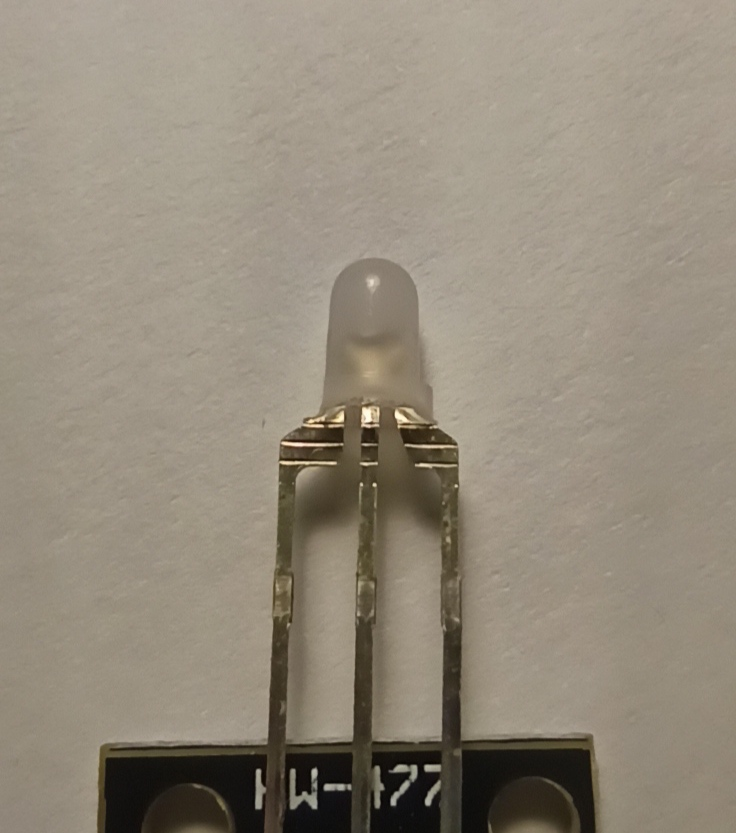
\includegraphics[width=.5\linewidth]{fig/HW-477/zdj_modułu/diodaLED.jpg}
\caption{Zdjęcie elementu diody RG LED}
\label{fig:_zdjecie_elementu}
\end{subfigure}%
%%%%%%%%%%%%%%%%%%%%%%%%%%%%%%%%%%%%%%%%%%%%%%%%%%%%%%%%%%%%%%%%%%%%%%%%%%%%%%%%%
\begin{subfigure}{.5\textwidth}
\centering
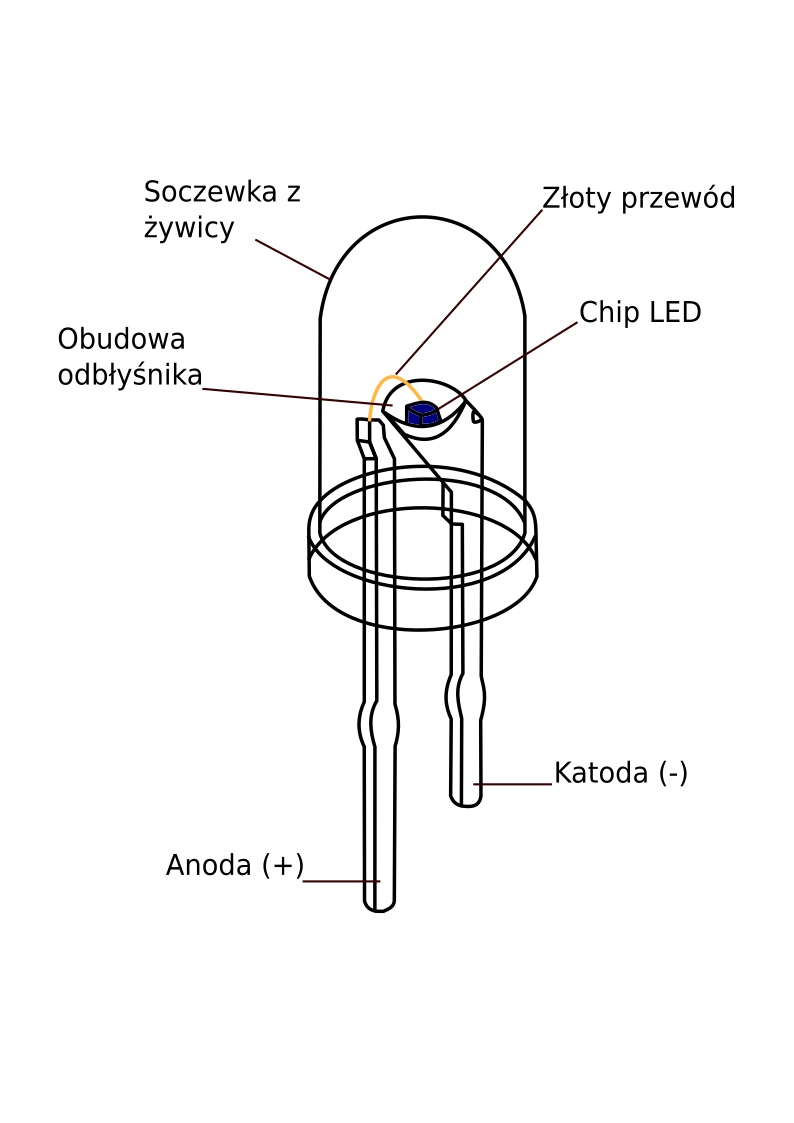
\includegraphics[width=.6\linewidth]{fig/HW-477/zasada_dzialania/rysunek.png}
\caption{LED - budowa elementu}
\label{fig:_zasada_dzialania_elementu}
\end{subfigure}
%%%%%%%%%%%%%%%%%%%%%%%%%%%%%%%%%%%%%%%%%%%%%%%%%%%%%%%%%%%%%%%%%%%%%%%%%%%%%%%%%
% \caption{PODPIS}
\label{fig:element}
\end{figure}
\vspace{0.25cm}
%%%%%%%%%%%%%%%%%%%%%%%%%  TWO IMAGES SIDE BY SIDE  %%%%%%%%%%%%%%%%%%%%%%%%%%%%%
% \subsection{Opis modułu} REPLACE SUBSECTION WITH 1CM VSPACE
\vspace{0.75cm}

Moduł HW-477 w zespole z diodą dwukolorową oferuje trzy piny: dwa umożliwiające sterowanie jedną z dwóch barw LED oraz jedno wyprowadzenie ujemne podpinane do masy.


%%%%%%%%%%%%%%%%%%%%%%%%%  TWO IMAGES SIDE BY SIDE  %%%%%%%%%%%%%%%%%%%%%%%%%%%%%
\begin{figure}[h]
\centering
%%%%%%%%%%%%%%%%%%%%%%%%%%%%%%%%%%%%%%%%%%%%%%%%%%%%%%%%%%%%%%%%%%%%%%%%%%%%%%%%%
\begin{subfigure}{.5\textwidth}
\centering
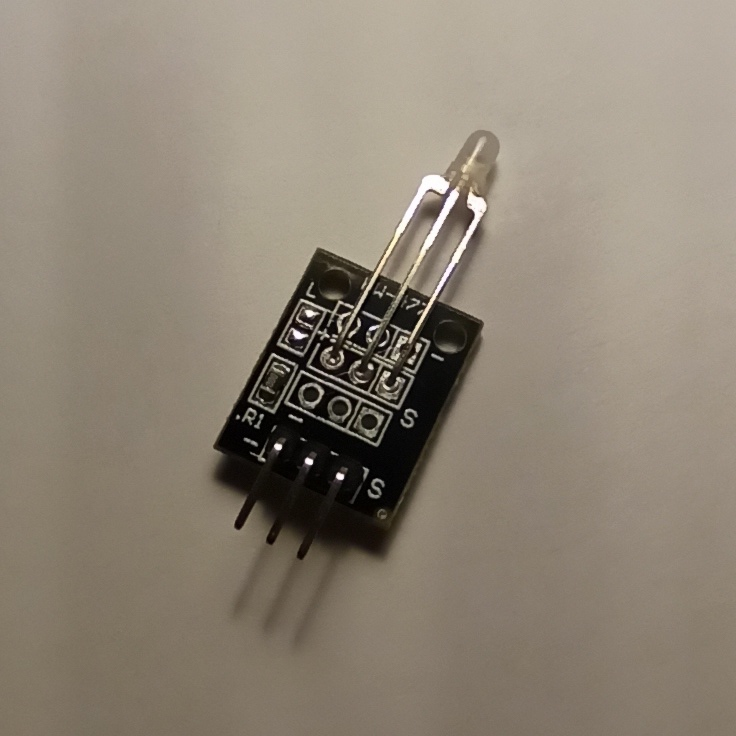
\includegraphics[width=.6\linewidth]{fig/HW-477/zdj_modułu/hw477_dualLED.jpg}
\caption{Zdjęcie modułu HW-477}
\label{fig:_zdjecie_modulu}
\end{subfigure}%
%%%%%%%%%%%%%%%%%%%%%%%%%%%%%%%%%%%%%%%%%%%%%%%%%%%%%%%%%%%%%%%%%%%%%%%%%%%%%%%%%
\begin{subfigure}{.5\textwidth}
\centering
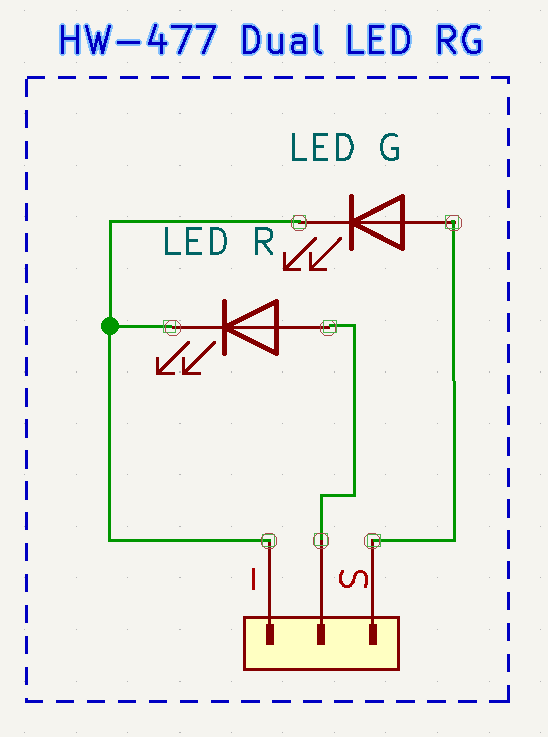
\includegraphics[width=.4\linewidth]{fig/HW-477/polaczenie_modulu/hw-477_dualLED_scheme.PNG}
\caption{Schemat modułu}
\label{fig:_schemat_modulu}
\end{subfigure}
%%%%%%%%%%%%%%%%%%%%%%%%%%%%%%%%%%%%%%%%%%%%%%%%%%%%%%%%%%%%%%%%%%%%%%%%%%%%%%%%%
\label{fig:modul}
\end{figure}
\vspace{0.5cm}
%%%%%%%%%%%%%%%%%%%%%%%%%  TWO IMAGES SIDE BY SIDE  %%%%%%%%%%%%%%%%%%%%%%%%%%%%%

\newpage
Taki element może mieć wiele zastosowań. Nie ma sensu wymieniać tu wszystkich, ale warto przytoczyć szczególne przypadki, w których ta konkretna dioda jest lepszym kandydatem niż konwencjonalna LED, czy rozszerzona o dodatkowy kanał LED RGB:
\vspace{0.5cm}
\begin{itemize}
    \item Urządzenia przemysłowe - wskaźnik świetlny stanu maszyny,
    \item Akumulatory - wskaźnik poziomu naładowania, 
    \item Zastosowanie w układach diagnostycznych - informowanie o poziomie cieczy w zbiorniku, prosty przekaz temepratury urządzenia, kolor diody informujący o stanie (np. wystąpienie błedu lub ostrzeżenia),
    \item Modelarstwo - czyli wszelakie aplikacje do pojazdów zdalnie sterowanych czy makiet
\end{itemize}
\vspace{0.5cm}
HW-477 Dual LED znajdzie swoje zastosowanie szczególnie w przypadkach, gdy w aplikacji potrzebna jest większa ilość barw światła przy jednoczesnym ograniczeniu potrzenych pinów wykorzystanych do jej obsługi.

\newpage

\section{Użycie modułu}
W celu najlepszego zaprezentowania układu, tutaj \cite{prezentacja} można przejść do bibliografii, w której znajduje się odnośnik do filmu prezentującego działanie układu mikrokontrolera STM32F7 z modułem HW-477 i diodą LED RG.

\vspace{0.5cm}
Działenie układu sprowadza się do cyklicznej zmiany stanów (HIGH/LOW) na wyjściach cyfrowych mikrokontrolera (PC8 oraz PC9). Konkretne wyjście odpowiada konkretnemu kolorowi światła diody. W pierwszej fazie poprzez ustawienie stanu HIGH na wyjściu PC8 uzyskujemy barwę czerwoną, następnie pin PC8 zmienia stań na LOW, a PC9 na HIGH - uzyskujemy barwę zieloną. Ostatecznie stan HIGH pojawia się na obu pinach - kolory się mieszają w barwę pomarańczową. Zmiany odbywają się w określonym odstępie czasowym. 

\vspace{0.5cm}
Połączenie mikrokontrolera z modułem zastosowane w przykładzie jest opisane w tabeli znajdującej się poniżej.

\vspace{0.5cm}
\begin{table}[h!]
    \centering
    \begin{tabular}{|c|c|c|c|} 
        \hline
        \multicolumn{2}{|c|}{NUCELO-F746ZG} & \multicolumn{2}{c|}{SENSOR}  \\ 
        \hline
        Etykieta & Port i numer pinu       & Nr pinu & Etykieta           \\ 
        \hline
        GND      & -                     & 1       & (-)              
        \\
        \hline
        D43      & PC8                     & 2       & R            
        \\
        \hline
        D44      & PC9                       & 3       & G              \\
        \hline
    \end{tabular}
    \caption{Połącznie pomiędzy modułem i mikrokontrolerem}
\end{table}

% TUTAJ FOTY ODNOSNIE TEGO
%%%%%%%%%%%%%%%%%%%%%%%%%  TWO IMAGES SIDE BY SIDE  %%%%%%%%%%%%%%%%%%%%%%%%%%%%%
\vspace{0.25cm}
\begin{figure}[h]
\centering
%%%%%%%%%%%%%%%%%%%%%%%%%%%%%%%%%%%%%%%%%%%%%%%%%%%%%%%%%%%%%%%%%%%%%%%%%%%%%%%%%
\begin{subfigure}{.5\textwidth}
\centering
\includegraphics[width=.9\linewidth]{fig/HW-477/działanie_ukladu/green.jpg}
\caption{Pin 3 w stanie HIGH - kolor zielony}
\label{fig:_uklad_woltomierz_otw}
\end{subfigure}%
%%%%%%%%%%%%%%%%%%%%%%%%%%%%%%%%%%%%%%%%%%%%%%%%%%%%%%%%%%%%%%%%%%%%%%%%%%%%%%%%%
\begin{subfigure}{.5\textwidth}
\centering
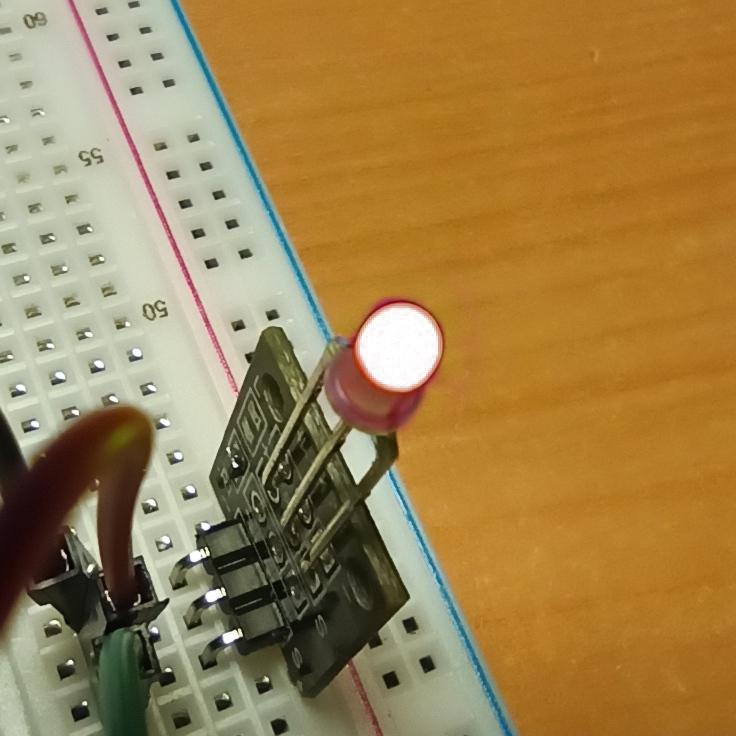
\includegraphics[width=.9\linewidth]{fig/HW-477/działanie_ukladu/red.jpg}
\caption{Pin 2 w stanie HIGH - kolor czerwony}
\label{fig:_uklad_woltomierz_zmk}
\end{subfigure}
%%%%%%%%%%%%%%%%%%%%%%%%%%%%%%%%%%%%%%%%%%%%%%%%%%%%%%%%%%%%%%%%%%%%%%%%%%%%%%%%%
% \caption{PODPIS}
\label{fig:woltomierz}
\end{figure}
\vspace{0.25cm}
%%%%%%%%%%%%%%%%%%%%%%%%%  TWO IMAGES SIDE BY SIDE  %%%%%%%%%%%%%%%%%%%%%%%%%%%%%

Dodatkowe schematy połączeń i konfiguracja
mikrokontrolera została opisana w sekcji \texttt{Suplement \#1}.Zawiera tam się również kod języka
C + HAL, pozwalający na obsługę modułu.

\newpage
\begin{figure}[h]
    \centering
    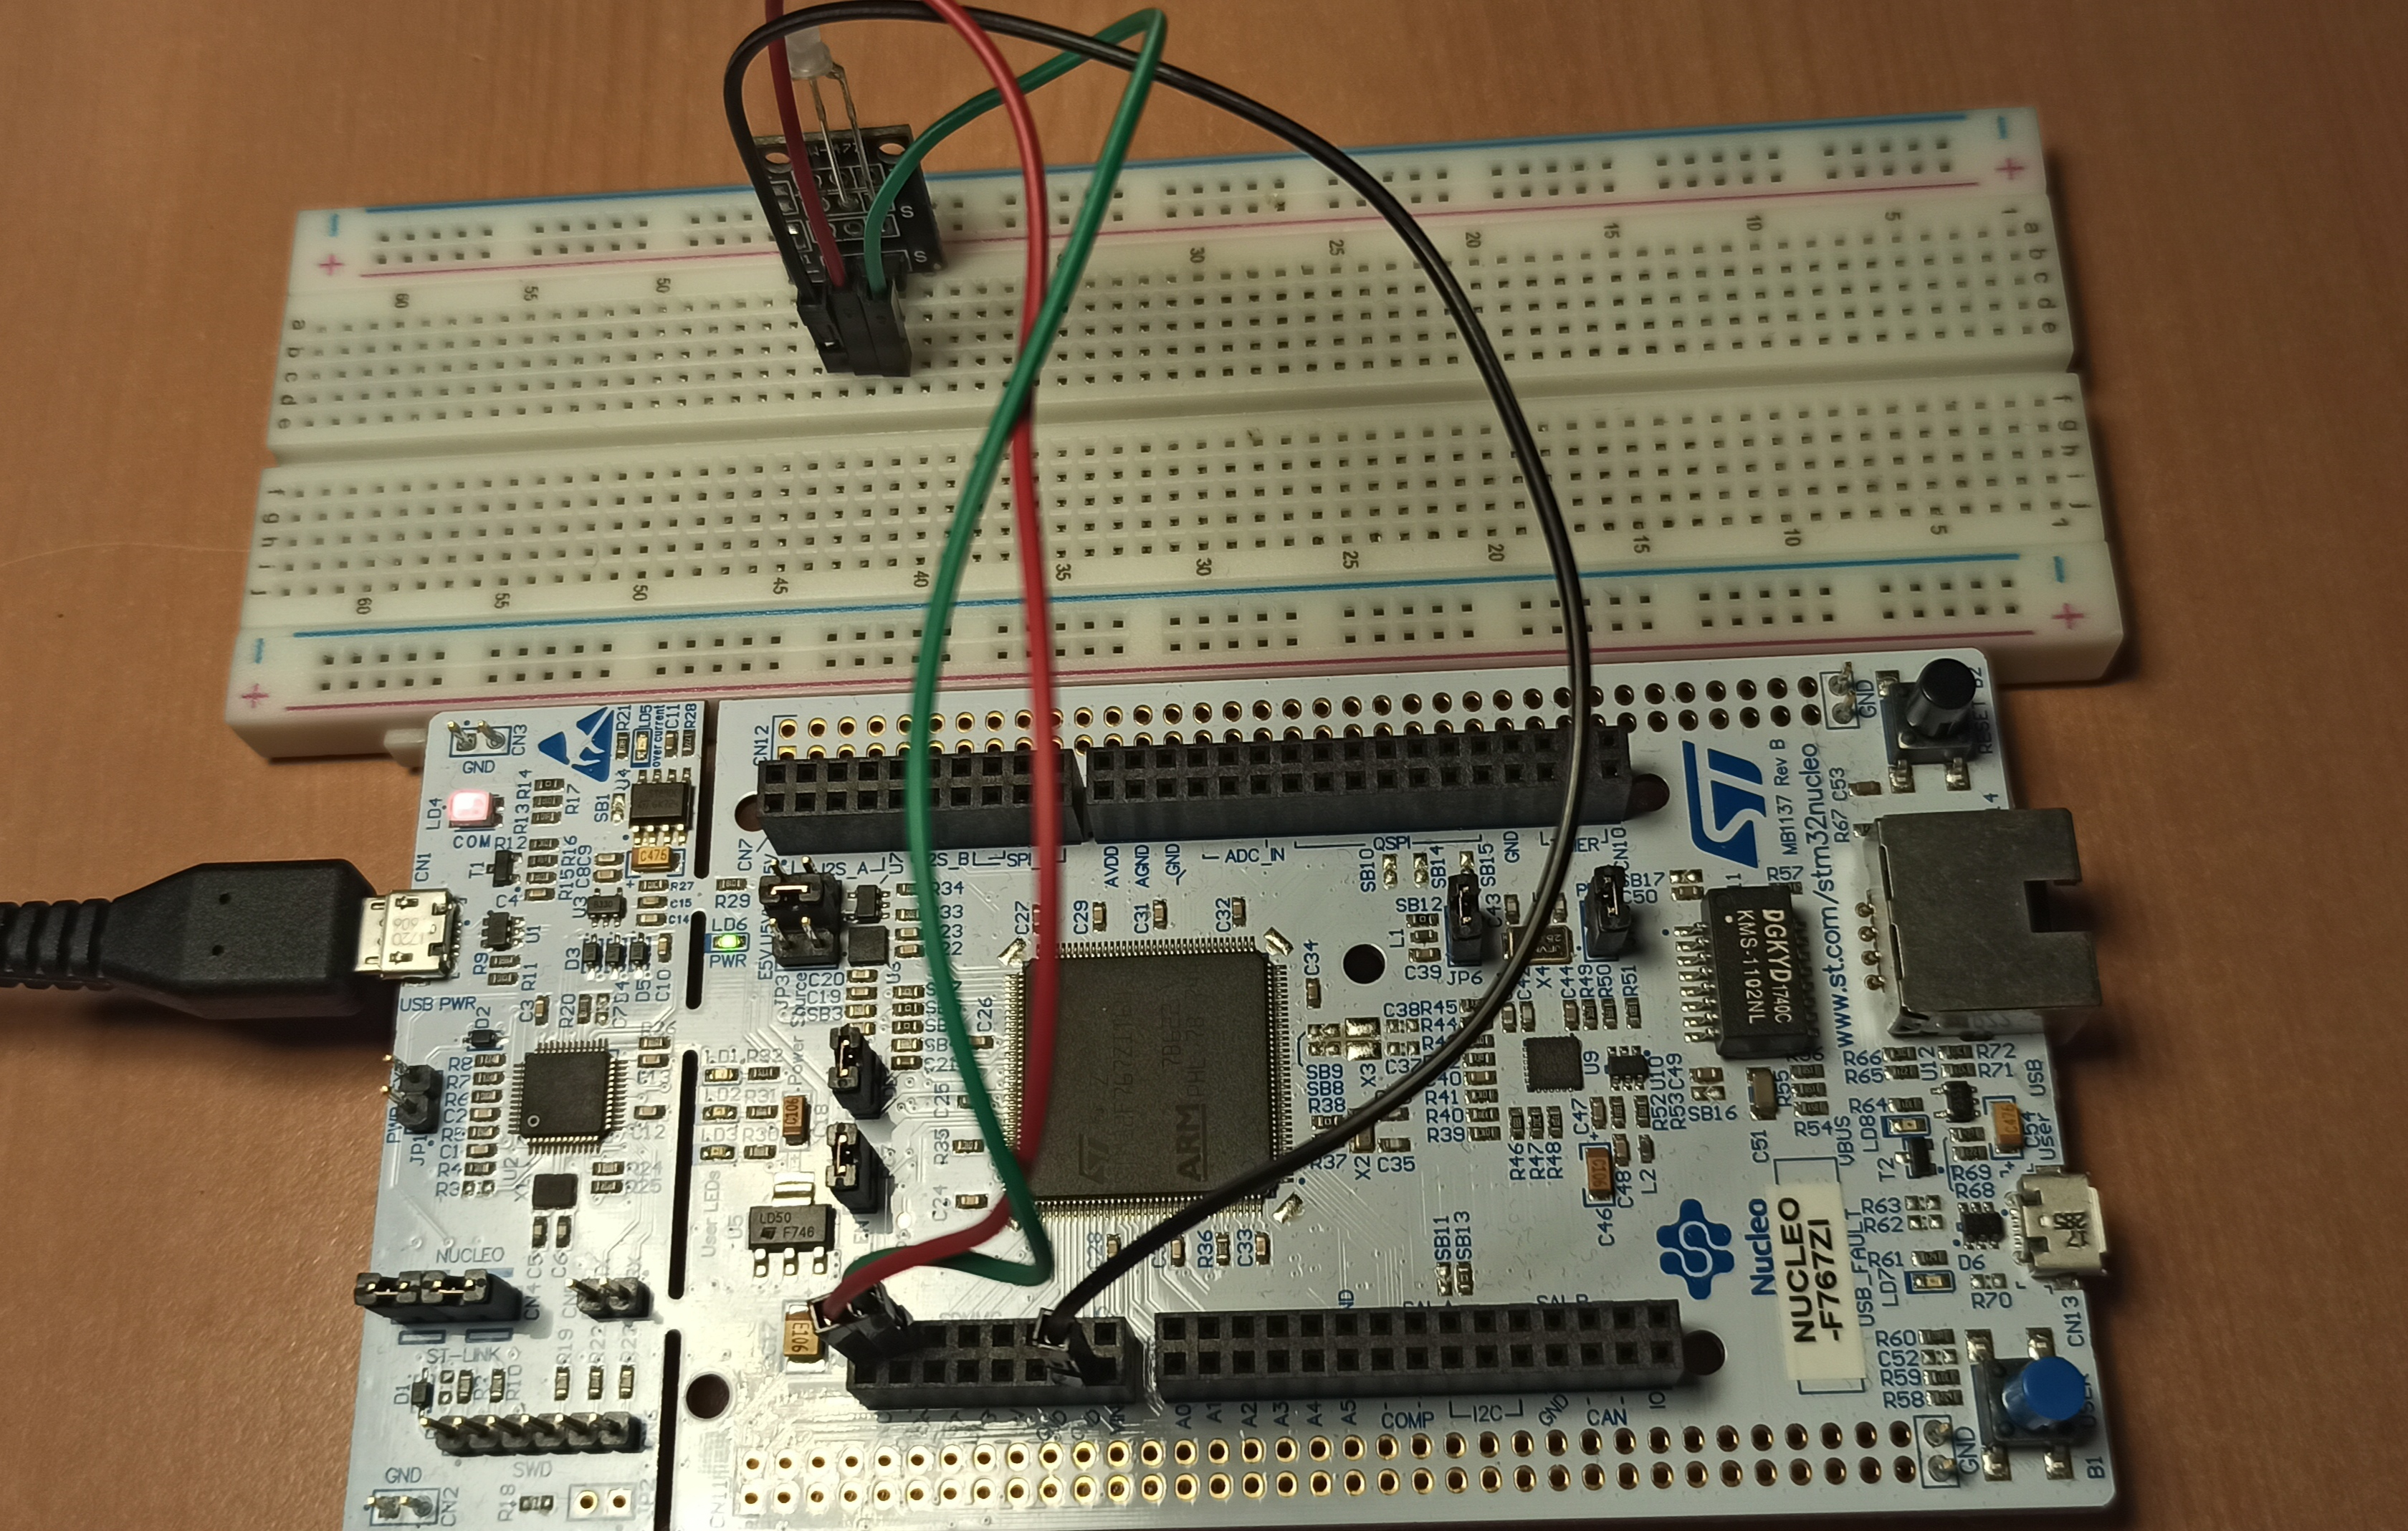
\includegraphics[width=0.65\textwidth]{fig/HW-477/działanie_ukladu/uklad1.jpg}
    \caption{Połączenie układu}
    \label{fig:polaczenie_ukladu}
\end{figure}

\begin{figure}[h]
    \centering
    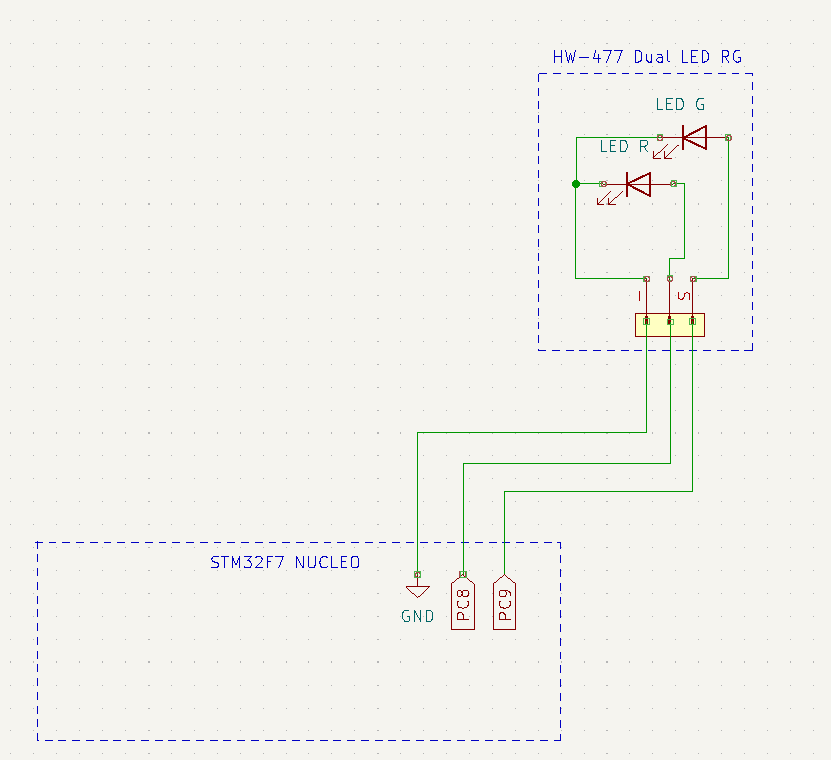
\includegraphics[width=0.6\textwidth]{fig/HW-477/polaczenie_modulu/hw-477_schemat2.PNG}
    \caption{Schemat połączenia układu}
    \label{fig:schemat_polaczenie_ukladu}
\end{figure}


Więcej informacji na temat kodu i oprogramowania zawarte jest w \texttt{Suplement \#1}.


Dodatkowo działanie układu przedstawiono na załączonym w \texttt{\cite{yt}} materiale 
wideo.

\newpage
\printbibliography[heading=bibintoc]

\end{document}